% Made up for the tikra benchmark.
\usetikzlibrary{circuits.logic.US, matrix, positioning, calc}
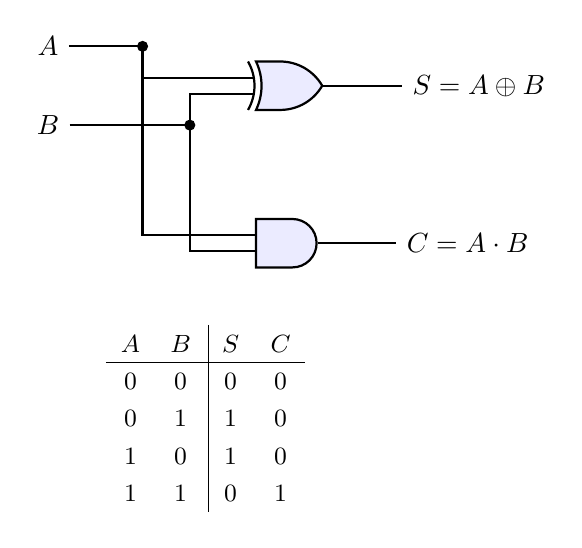
\begin{tikzpicture}[circuit logic US, thick, every circuit symbol/.style={fill=blue!8}]
  \node[xor gate, inputs=nn] (xor) at (3,1) {};
  \node[and gate, inputs=nn] (and) at (3,-1) {};
  \node (a) at (0,1.5) {$A$};
  \node (b) at (0,0.5) {$B$};
  \draw (a) -- (1.2,1.5) |- (xor.input 1);
  \draw (b) -- (1.8,0.5) |- (xor.input 2);
  \draw (1.2,1.5) |- (and.input 1);
  \draw (1.8,0.5) |- (and.input 2);
  \fill (1.2,1.5) circle (2pt) (1.8,0.5) circle (2pt);
  \draw (xor.output) -- ++(1,0) node[right] {$S = A \oplus B$};
  \draw (and.output) -- ++(1,0) node[right] {$C = A \cdot B$};
  \matrix[below=6mm of and.south, xshift=-1cm, matrix of math nodes, nodes={minimum width=6mm},
      column sep=1pt, row sep=1pt, font=\small] (tt) {
    A & B & S & C \\
    0 & 0 & 0 & 0 \\
    0 & 1 & 1 & 0 \\
    1 & 0 & 1 & 0 \\
    1 & 1 & 0 & 1 \\
  };
  \draw[thin] (tt-1-1.south west) -- (tt-1-4.south east);
  \draw[thin] (tt-1-2.north east) ++(1pt,0) -- ($(tt-5-2.south east)+(1pt,0)$);
\end{tikzpicture}
